 
\chapter{Cellular phenomena}
\label{chap:cellular-phenomena}


\section{Refractory period}
\label{sec:refractory-period}

\section{Self-oscillation in cardiac myocardium}

\url{https://en.wikipedia.org/wiki/Self-oscillation}

\url{https://en.wikipedia.org/wiki/Autowave}


The classical axiomatic model with autowaves in myocardium was published in 1946
by Norbert Wiener and Arturo Rosenblueth.


\section{HAP, AHP, and DAP}
\label{sec:hap-ahp-dap}

\begin{figure}[hbt]
  \centerline{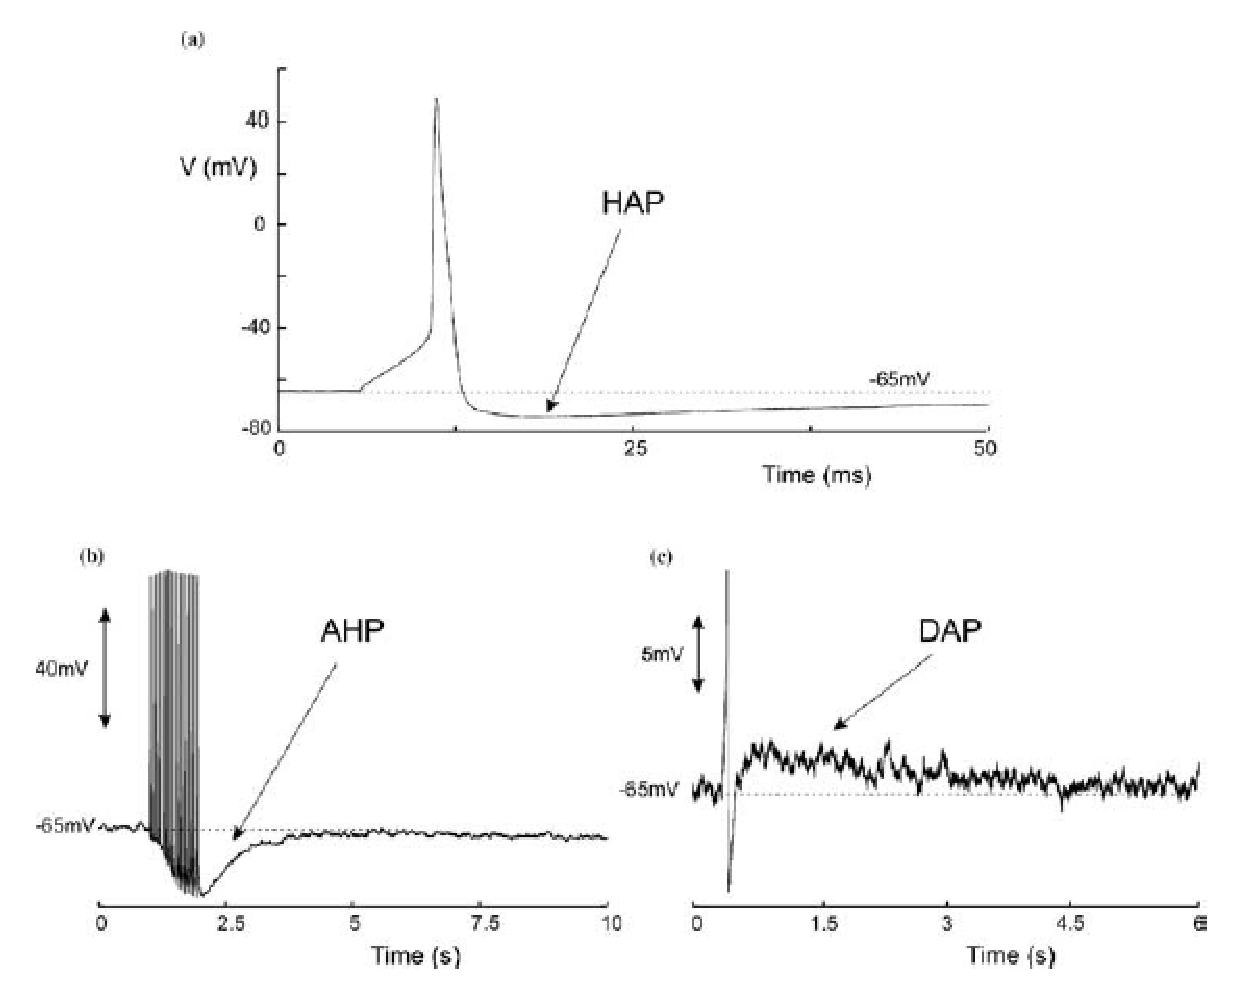
\includegraphics[height=8cm,
    angle=0]{./images/AHP_HAP_DAP.eps}}
\caption{HAP, AHP and DAP in magnocellular neurosecretory cells}
\label{fig:HAP_AHP_DAP}
\end{figure}

\begin{itemize}
\item HAP = hyperpolarized after-potential (negative after-potential
  compared to resting potential)
\item AHP = after-hyperpolarizing potential 
\item DAP = depolarized after-potential (positive after-potential
  compared to resting potential)
\end{itemize}

HAP and DAP are classified into early after-potential (EAP); while AHP
is classified into late after-potential (LAP).

\section{[Early] Afterpotential (EAP)}
\label{sec:afterpotential}

{\bf Early afterpotential} is the action potential (AP) with smaller
AP duration (APD), the relatively small repolarization/depolarization,
generated following the termination of the main AP (the spike). If it
is repolarization, we have negative after-potential or hyperpolarized
after-potential (HAP); otherwise, we have positive after-potential or
depolarized afterpotential (DAP) compared to the resting potential.

Normally, the early afterpotential is HAP. However, if the resting
potential was quite negative, the negative after-potential was
replaced by a positive after-potential, i.e. the spike terminates in
the phase of hyperpolarization.

In rat muscle, the afterpotential was always smallest in the first
spike of a burst and it increases gradually with the repetition of
discharge. Also, it was suggested that the negative after-potential is
largely due to an increase in \ce{Cl} conductance of the membrane,
which cause depolarization, or a delay in
repolarization~\citep{ohashi1970eci}.

\subsection{HAP (hyperpolarized after-potential)}
\label{sec:hap-hyperp-after}

As shown in Fig.~\ref{fig:HAP_AHP_DAP}

\subsection{DAP (depolarized afterpotential)}
\label{sec:dap-depol-afterp}

DAP is the phenomenon of a second small pump (of membrane depolarization)
after an action potential, e.g. in CA1 neuron. The amplitude of the depolarizing
after AP depends on potassium conductance, as shown in Fig.~\ref{fig:DAP}.
\begin{figure}[hbt]
  \centerline{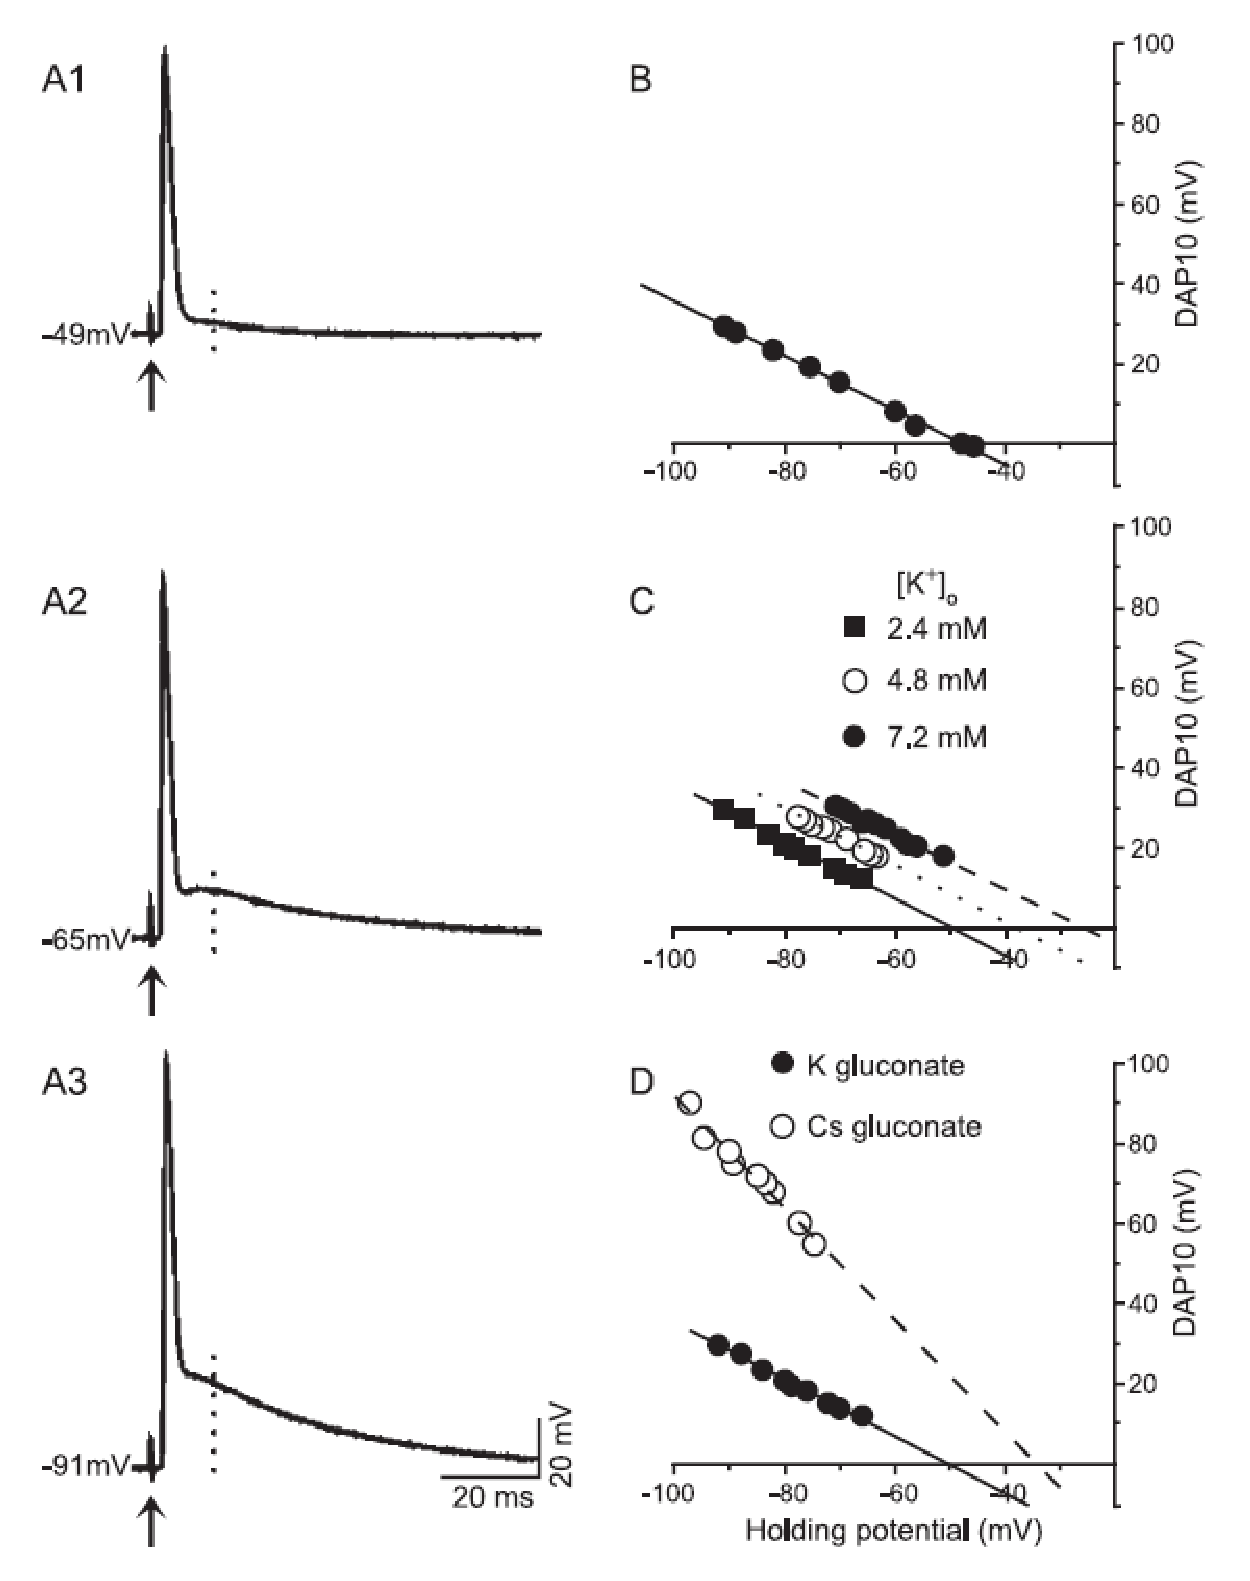
\includegraphics[height=8cm,
    angle=0]{./images/DAP.eps}}
\caption{The amplitude of DAP after 10ms of the AP (DAP10); it
  increases with holding potential (A) -49mV, (B) -65mV, (C) -91mV}
\label{fig:DAP}
\end{figure}

DAP of large magnitude have not been previously described in
CNS. Several hypothesises derived to explain the classical DAP in
axons. 
\begin{itemize}
\item DAP relates to a diffusion barrier surrounding the axon. This
  barrier causes \ce{K+} leaving the cell during the late phase of the
  spike, to accumulate near external membrane surface. Then, the
  depolarizing action of the accumulated \ce{K+} is responsible for
  DAP. This accumulation hypothesis requires (1) repetitive firing
  produce a cumulative DAP, (2) decay of DAP be exponential, (3) time
  constant of the decay be independent of the number of spikes in a
  burst~\citep{kandel1961ehn_b}, as shown in
  Fig.~\ref{fig:repetitive_firing}.
\item increase in \ce{Na+} conductance 
\item passive decay of soma membrane potential following the transient
  increase of conductance associated with the spike
\end{itemize}
The two latter hypothesises are used to explain DAP for a single
spike. 

\begin{figure}[hbt]
  \centerline{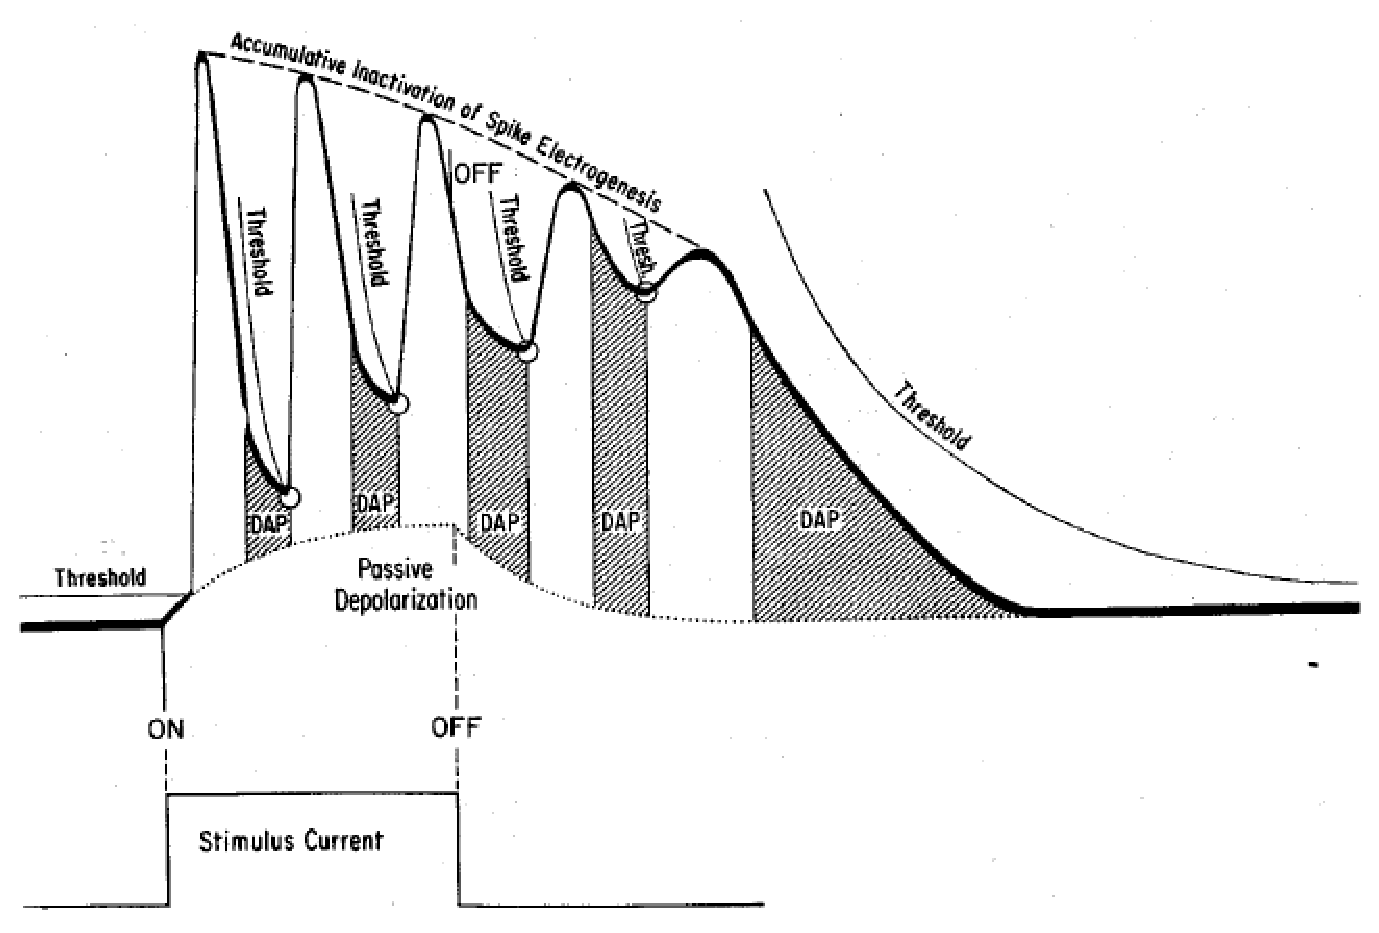
\includegraphics[height=5cm,
    angle=0]{./images/repetitive_firing.eps}}
\caption{Schematic diagram of a repetitive firing }
\label{fig:repetitive_firing}
\end{figure}



\section{[Late] after-potential (LAP)}
\label{sec:late-after-potential}

LAP refers to an AP of longer AP duration (APD).  In frog skeletal
muscle, Freygang et al. (1964) suggested that LAP is caused by
accumulation of potassium inside the T-tubule system. It means that K
channels should reside on T-tubule system also. This was tested and
validated by Kirsch et al.~\citep{kirsch1977drtt}.

Most models only consider L-type channels and RyR channels in a
release site (CaRU). Thus, \textcolor{red}{the idea is to take into
  account potassium channels in the release site} in cardiac
myocytes??? This is a good idea if we consider muscle cells. However,
with cardiac cells, we don't have K channels in the T-tubule. 


\subsection{AHP (after-hyperpolarization)}
\label{sec:ahp-after-hyperp}

Action potential afterhyperpolarization (AHP) refers to the prolonged
depolarization after an AP. AHP enhances precision of firing by ensuring that
the ion channels recover from inactivation by the same amount on each cycle. 
AHP is often observed in bursting behavior (Sect.\ref{sec:bursting_behavior}).

After repetitive firing (spontaneous \ce{Ca^2+} spikes), or {\bf burst}, in the
hippocampal CA1 neuron, we observe long-lasting after-hyperpolarization (AHP),
as shown in Fig.~\ref{fig:AHP}~\citep{hotson1980ahp}.
AHP may persists for several seconds and thus may have profound consequences for
the firing pattern of the neuron. The AHP has several components with different
time courses.  

% :
% one fAHP (Sect.\ref{sec:AHP-fast}) and one or many sAHP (Sect.\ref{sec:AHP-slow}).


\begin{enumerate}
  \item fast AHP:   markedly reduced by low concentrations of 4-aminopyridine
  (Sect.\ref{sec:4-AP}) and $\alpha$-dendrotoxin ($\alpha$-DTX -
  Sect.\ref{sec:dendrotoxin}), indicating the involvement of voltage-gated
  potassium channels 

  \item medium AHP: blocked by apamin and UCL1848, indicating it
was mediated by small conductance calcium-activated potassium
channel (SK) channels - Sect.\ref{sec:SK_current}

  \item slow AHP: mediated by non-SK BK channels, was apamin-insensitive, but
  was modulated by carbachol and noradrenaline.
\end{enumerate} 

Observations:
\begin{itemize}
\item AHP is unaffected by:
  \begin{enumerate}
  \item the increase in intracellular \ce{Cl-}
  
  \item \ce{Na+} potentials, i.e. \ce{Na+} influx is blocked by
    tetrodotoxin (TTX) $\rightarrow$ \ce{Ca^2+} is resisted to TTX, or
    we can say TTX-resistant \ce{Ca^2+} spikes.
  \end{enumerate}
  
\item Block AHP (or short-duration AHP) if:

  \begin{enumerate}
  \item reduce [\ce{K+}] conductance, by using \ce{K+}-channel
    blocker, e.g. \ce{Ba^2+}

  \item calcium influx is blocked by using \ce{Ca^2+} inhibitor,
    e.g. \ce{Mn^2+}
  \end{enumerate}
\end{itemize}

One possible explaination for the mechanism for the different AHP time courses
might be if the kinetics of gating were different for the channels underlying
each type of AHP. 

Each component of the AHP is kinetically distinct and is mediated by different
Ca2+-activated K+ channels. In the case of sAHP, there are three different K+
channels: SK1, SK2 and SK3. However, since steady state calcium gating is not
different for cloned apamin-sensitive (SK2, SK3) or apamin-insensitive (SKI)
channels, it is unlikely that the kinetics of calcium activation of these
channels is different.
Thus, it suggests he kinetic differences of the sAHPs reflects different rates
of calcium exposure.
 
However, blockade of large
conductance calciumactivated potassium channel (BK) channels
(Sect.\ref{sec:AHP-fast}) with paxilline, iberiotoxin, or TEA revealed that BK
channels are involved in action potential repolarization but only make a small
contribution to the fast AHP that follows action potentials.

% The time period of AHP is the duration of inhibitory postsynaptic potential
% (IPSP)

\begin{figure}[hbt]
  \centerline{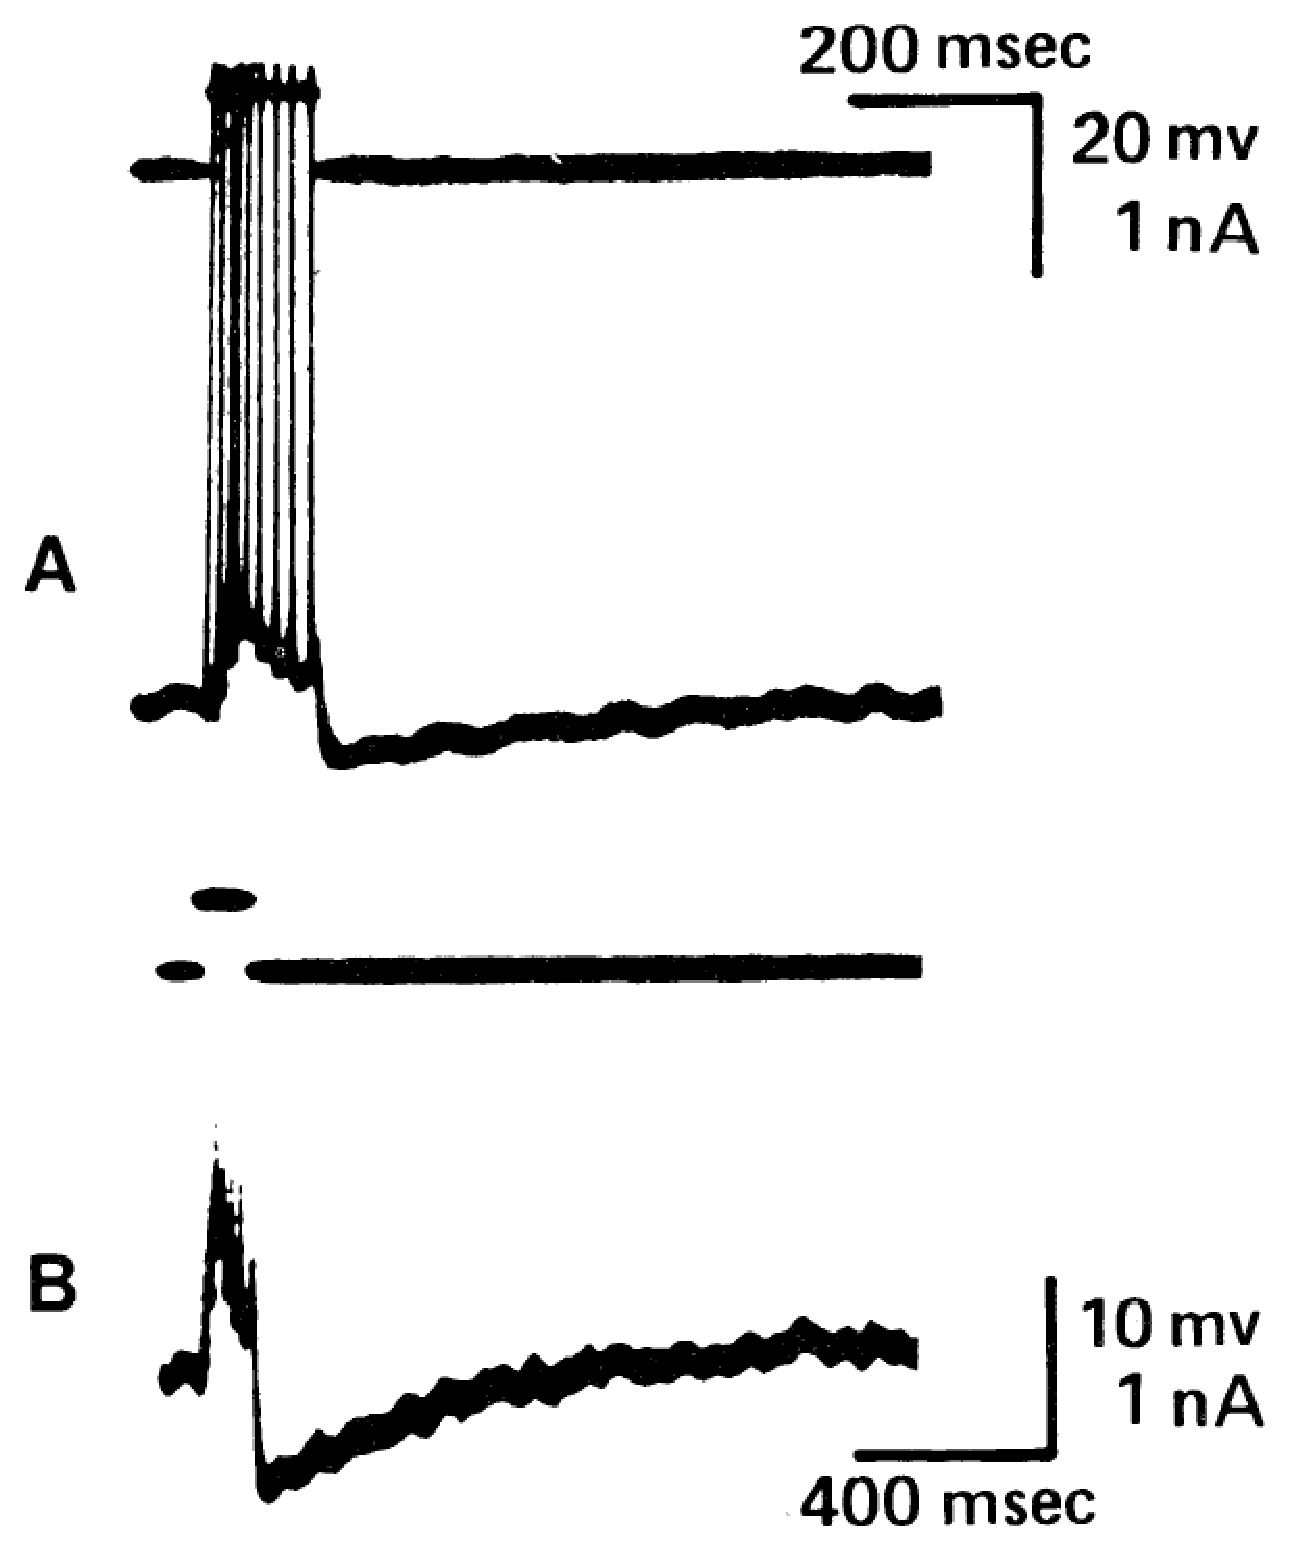
\includegraphics[height=5cm,
    angle=0]{./images/AHP.eps}}
\caption{current-induced repetitive firing followed long-lasting AHP ($E_r=-60$mV)~\citep{hotson1980ahp}}
\label{fig:AHP}
\end{figure}


AHP is mediated by an increase in \ce{K+} conductance after a
spontaneous burst. This burst occurs after \ce{Ca^2+} influx. It is
thus believed that \ce{Ca^2+}-activated increase \ce{K+} conductance,
or there is \ce{Ca^2+}/\ce{K+} coupling.

AHP is required to repolarize a repetitive firing cell to its normal
resting potential value. The long-lasting AHP appears to be maximally
activated by rapidly cellular firing and in the termination of
spontaneous bursts of repetitive discharges. 

References:


\subsection{-- fAHP (fast AHP)}
\label{sec:AHP-fast}) 

The fast component (fAHP) helps to repolarize the action potential and regulates spike
interval. fAHP is mediated by the large-conductance (100 to 200 pS), voltage-
and  Ca2+-activated K+ channels (BK channels) - Sect.\ref{sec:BK-current}.

The fAHP is blocked by low concentration of external tetraethylammonium and
charybdotoxin, in accord with the pharmacology of BK channels.


\subsection{-- sAHP (slow AHP): apamin-sensitive sAHP (mAHP) or
apamin-insensitive sAHP} \label{sec:AHP-slow}).

There are one or many subsequent slow components (sAHP) during an AHP and they
underlie spike-frequency adaptation. Slow AHPs can be classified into two 
groups,  based  on  level of sensitivity  to  the bee  venom  toxin  {\bf
apamin}.

% The sAHP exhibits one or the other of two classes of behavior regarding
% sensitivity to the bee venom peptide toxin apamin.

There are two types of sAHP (described as follows). The two classes of sAHPs are
not mutually exclusive, i.e. they are frequently coexpressed as in rat and
guinea pig vagal neurons, cat, and rat cortical neurons, and guinea pig
cholinergic nucleus basalis neurons  both apamin-sensitive and
apamin-insensitive AHPs are present.
Each type correspond to the action of a different SK channel: apamin-sensitive
SK (Sect.\ref{sec:SK_current-apamin-sensitive}) and apamin-insensitive SK
(Sect.\ref{sec:SK_current-apamin-insensitive})

\begin{enumerate}
  \item  \textcolor{red}{apamin-sensitive sAHPs} (also {\bf NOT regulated by
  neurotransmitter-induced second messengers}) activate rapidly following a
  single action potential and decay with a time constant of approximately 150 ms.

Apamin-sensitive sAHPs have faster kinetics than apamin-insensitive sAHP.
In some cells, such as in hippocampal interneurons, guinea pig trigeminal
motoneurons, or septal  cholinergic  neurons, the  apamin-sensitive 
sAHP  is  maximal  following  an  action potential and decays with a half-time
on the order of hundreds of milliseconds.

In hippocampal pyramidal neurons the sAHP is insensitive to apamin, whereas
in hippocampal interneurons it is blocked by nanomolar concentrations of 
apamin (Kohler et al., 1996). 

  \item  \textcolor{red}{apamin-insensitive sAHPs} (also regulated by
  neurotransmitter-induced second messengers) rise slowly and decay with a time
  constant of approximately 1.5 seconds.

Apamin-insensitive sAHPs are relatively rare, but have been well documented in
hippocampal pyramidal neurons, where apamin application does not affect the
sAHP. Also, apamin-insensitive sAHPs are found in  septal  cholinergic,
neocortical, and  sensorimotor  neurons.

Noradrenaline, dopamine, serotonin, histamine, acetylcholine  (via  muscarinic
receptors)  and  glutamate  (via  metabotropic  receptors),  as well as some
neuropeptides (VIP, CRF), all suppress the apamin-insensitive sAHP, i.e.
neuronal  excitability  is  enhanced,  spike  frequency  adaptation  is 
strongly decreased, and the number of action potentials evoked by a certain
depolarizing stimulus is increased.

In contrast, adenosine can decrease neuronal excitability by increasing the
apamin-insensitive sAHP.

\end{enumerate}

The distinction between fAHP vs sAHP in terms of time scale of kinetics is also
seen in cells that  have  two  distinct  kinetic  phases  to  the  sAHP: a
relatively  faster,  apamin-sensitive phase, sometimes referred to as the
medium, or mAHP; and a relatively slower apamin- insensitive phase, the sAHP.

Typically, the difference in stimulus paradigm determine which one occurs.
Example: in rat hypoglossal motoneurons, cholinergic nucleus basalis neurons, or
basal forebrain neurons
\begin{itemize}
  
  \item the apamin-sensitive mAHP may be evoked by a single or a short burst of
  action potentials.
  
  \item the long-lasting apamin-insensitive sAHP (in the same cells as above)
  can only be triggered by long trains of action potentials
\end{itemize}


%%% Local Variables: 
%%% mode: latex
%%% TeX-master: "mainfile"
%%% End: 

